\documentclass[11pt]{article}
\usepackage[parfill]{parskip}
\usepackage{tikz, amsmath, amssymb, graphics, setspace, geometry, mathtools, fancyhdr, hyperref, expl3, fancyvrb, listings, xfp}

\newcommand{\eps}{\epsilon}
\newcommand{\mysum}{\displaystyle \sum}
\newcommand{\myprod}{\displaystyle \prod}
\newcommand{\ceil}[1]{\left \lceil{#1}\right \rceil}
\newcommand\tab[1][1cm]{\hspace*{#1}}
\newcommand{\N}{\mathbb{N}}
\newcommand{\Z}{\mathbb{Z}}

\edef\getxnow(#1,#2){#1}
\edef\getynow(#1,#2){#2}
\newcommand*{\getx}[1]{\expandafter\getxnow#1}
\newcommand*{\gety}[1]{\expandafter\getynow#1}

\newcommand*{\scalePic}{0.4}
\newcommand*{\gridArg}[7]{% xstart, xdiff, xend, ystart, ydiff, yend, visibility (possibly empty)
    \foreach \x in {\fpeval{#1},\fpeval{#1+#2},...,\fpeval{#3+0.0001}} % + 0.0001 to avoid chopping off the final coordinate when using floating-point coordinates
        \draw [black, thin, #7] (\x,\fpeval{#4}) -- (\x,\fpeval{#6+0.0001});
    \foreach \y in {\fpeval{#4},\fpeval{#4+#5},...,\fpeval{#6+0.0001}}
        \draw [black, thin, #7] (\fpeval{#1},\y) -- (\fpeval{#3+0.0001},\y);
}
\newcommand*{\grid}[6]{\gridArg{#1}{#2}{#3}{#4}{#5}{#6}{}}% xstart, xdiff, xend, ystart, ydiff, yend
\newcommand*{\phantombox}[4]{\gridArg{#1}{#3}{#1+#3}{#2}{#4}{#2+#4}{draw=none}} % xstart, ystart, xdiff, ydiff
\newcommand*{\mybigbox}[4]{\grid{#1}{#3}{#1+#3}{#2}{#4}{#2+#4}} % xstart, ystart, xdiff, ydiff
\newcommand*{\mybox}[2]{\mybigbox{#1}{#2}{1}{1}} % xstart, ystart (goes 1 in each direction)
\newcommand*{\myboxes}[1]{\foreach \pt in {#1} {\mybox{\getx{\pt}}{\gety{\pt}}}}
\newcommand*{\point}[3]{\node at (#1 + 0.5, #2 + 0.5)[circle, fill, inner sep=\scalePic*5pt, #3]{}; \gridArg{#1}{1}{#1+1}{#2}{1}{#2+1}{draw=none}}
\newcommand*{\labelabove}[3]{\node[above, outer sep=5pt] at (#1 + 0.5, #2 + 0.5){#3};} % x, y, label
\newcommand*{\red}{red!80!blue}
\newcommand*{\orange}{orange}
\newcommand*{\black}{black}
\newcommand*{\green}{green!70!blue}
\newcommand*{\blue}{blue!60!green}
\newcommand*{\brown}{brown}
\newcommand*{\white}{white}
\newcommand{\allcolor}[1]{%
  \expandafter\gdef\csname all#1\endcsname##1{%
    \foreach \pt in {##1} {\point{\getx{\pt}}{\gety{\pt}}{\csname #1\endcsname}}%
  }%
}
\newcommand{\allcolors}[1]{\foreach \r in {#1} {\expandafter\allcolor\expandafter{\r}}}
\allcolors{blue, orange, brown, red, black}

% Rewrites input text to be inside a lstlisting block when this is executed within a shell, and the shell's output is parsed as LaTeX input.
% lstlisting is like verbatim but offers word wrap. Useful for displaying error messages from shells.
\newcommand{\echoWithinShell}[1]{ ( echo \\\\\\\\begin\\{lstlisting\\}\\[breaklines\\] && echo #1 && echo \\\\\\\\end\\{lstlisting\\} ) }

\ExplSyntaxOn
\NewDocumentCommand{\getFromShell}{mm}
 {% #1 = command, #2 = control sequence to define
  \sys_get_shell:nnN { #1 } { } #2
  \tl_trim_spaces:N #2
 }
 \exp_args_generate:n{en}
\NewDocumentCommand{\defFromShellRun}{mmm}
 {%, shell command, desc for failure, new LaTeX command to define
  \exp_args:Nen\getFromShell{OUTPUT=`#1~2>&1`~&&~echo~$OUTPUT~||~(~\echoWithinShell{Failed~to~#2:}~&&~\echoWithinShell{\\~#1}~&&~\echoWithinShell{\\~$OUTPUT}~)} { #3 }
 }
\ExplSyntaxOff

% NOTE: need to enable shell escape in LaTeX settings to use \input{|...} which calls out to a system shell
\newcommand{\shellRun}[2] {% cmd, desc for failure
  \input{|OUTPUT=`#1 2>\&1` && echo $OUTPUT || ( \echoWithinShell{Failed to #2:} && \echoWithinShell{\\ #1} && \echoWithinShell{\\ $OUTPUT} ) }%
}

\newcommand{\cppCompileAndCleanup}[2] {% src, exe
  \shellRun{clang++ #1 -std=c++17 -o #2}{compile}
  \AtEndDocument{\input{| rm #1 #2}}
}
\newcommand{\cppRun}[2]{% exe, runtime args
  \shellRun{#1 #2}{run}
}


\pagestyle{fancy}
\lhead{David Fink}
\chead{Order from Infinite Chaos}
\rhead{Page \thepage}

\begin{document}

\title{Order from Infinite Chaos}
\author{David Fink}
\maketitle{}


\section*{Problems}

% NOTE: need to add the following line to the end of texmf.cnf (on my machine, /usr/local/texlive/2021/texmf.cnf ) - find location in a Terminal via "kpsewhich texmf.cnf"
% openout_any=a
% This allows LaTeX to write to files outside the folder where the current .tex file lives.
\getFromShell{kpsewhich -expand-var=$TMPDIR}{\tmpdir}
\newcommand{\src}{\tmpdir/my_cppFromLaTeX.cpp}
\newcommand{\exe}{\tmpdir/my_cppExeFromLaTeX.runme}
\begin{VerbatimOut}{\src}
#include <iostream>
#include <sstream>
#include <optional>
#include <vector>

using Coordinate = double;

struct Pt {
  Coordinate fX;
  Coordinate fY;
};

using Color = std::string;

struct Box {
    Pt fStart;
    Pt fSizes;
};

struct Shape {
    std::vector<Pt> fBase;
    Pt fNew;
};

struct Drawing {
  private:
    std::vector<std::pair<Pt, Color>> fPoints;
    std::vector<Box> fBoxes;
    Coordinate fSize;

  private:
    Drawing() = default;

  public:
    Drawing(Color initColor)
        : fPoints{{{0, 0}, initColor}}
        , fBoxes{{{0, 0}, {1, 1}}}
        , fSize(0) {
    }
    Drawing apply(Shape const& s, Coordinate scale, Color const& newPtColor) const {
        Drawing newD;
        for (auto const& [dx, dy] : s.fBase) {
            for (auto const& [pt, c] : fPoints) {
                auto [x, y] = pt;
                newD.fPoints.push_back({{x + dx * scale, y + dy * scale}, c});
            }
            for (auto const& box : fBoxes) {
                auto [x, y] = box.fStart;
                auto [boxdx, boxdy] = box.fSizes;
                newD.fBoxes.push_back({{x + dx * scale, y + dy * scale}, {boxdx, boxdy}});
            }
        }

        // add new pt
        auto newSize = fSize + scale;
        auto newPt = s.fNew;
        auto newPtx = newPt.fX * newSize;
        auto newPty = newPt.fY * newSize;
        newD.fPoints.push_back({{newPtx, newPty}, newPtColor});

        // add new box
        auto minCoord = newD.fPoints[0].first.fX;
        auto maxCoord = minCoord;
        for (auto const& [pt, c] : newD.fPoints) {
            auto [x, y] = pt;
            maxCoord = std::max(maxCoord, x);
            maxCoord = std::max(maxCoord, y);
            minCoord = std::min(minCoord, x);
            minCoord = std::min(minCoord, y);
        }
        newD.fBoxes.push_back({{0, 0}, {maxCoord + 1, maxCoord + 1}});
        
        newD.fSize = newSize;
        
        return newD;
    }
    
    std::string toString() const {
        std::ostringstream oss;
        for (auto const& [pt, color] : fPoints) {
            auto [x, y] = pt;
            oss << "\\\\point" << '{' << x << '}' << '{' << y << '}' << '{' << "\\\\" << color << '}' << std::endl;
        }
        for (auto const& box : fBoxes) {
            auto [x, y] = box.fStart;
            auto [dx, dy] = box.fSizes;
            oss << "\\\\mybigbox{" << x << "}" << "{" << y << "}" << "{" << dx << "}" << "{" << dy << "}" << std::endl;
        }
        return oss.str();
    }
};

[[nodiscard]] static bool consume(std::istream& is, char c) {
    std::ws(is);
    if (is.peek() == c) {
        is.get();
        return true;
    } else {
        return false;
    }
}

[[nodiscard]] static bool consume(std::istream& is, std::string const& s) {
    for (char c : s) {
        if (std::isspace(c)) {
            // ignore
        } else if (!consume(is, c)) {
            return false;
        }
    }
    return true;
}

[[nodiscard]] static std::optional<Coordinate> consumeCoordinate(std::istream& is) {
    Coordinate x;
    is >> x;
    if (is.fail()) {
        return std::nullopt;
    }
    return x;
}

[[nodiscard]] static std::optional<Pt> consumePt(std::istream& is) {
    if (!consume(is, '(')) {
        return std::nullopt;
    }
    auto optX = consumeCoordinate(is);
    if (!optX) {
        return std::nullopt;
    }
    auto x = *optX;
    if (!consume(is, ',')) {
        return std::nullopt;
    }
    auto optY = consumeCoordinate(is);
    if (!optY) {
        return std::nullopt;
    }
    auto y = *optY;
    if (!consume(is, ')')) {
        return std::nullopt;
    }
    return Pt{x, y};
}

[[nodiscard]] static std::optional<Color> consumeColor(std::istream& is) {
    std::ws(is);
    std::string result;
    while (!std::isspace(is.peek()) && !std::isdigit(is.peek()) && !is.eof()) {
        result += is.get();
    }
    if (result.empty()) {
        return std::nullopt;
    }
    return result;
}

int main(int argc, char** argv) {
    std::string args;
    for (int i = 1; i < argc; ++i) {
        args += std::string(" ") + argv[i];
    }
    std::istringstream is(args);

    std::vector<Pt> basePts;
    if (!consume(is, '{')) {
        std::cerr << "Missing expected open curly brace" << std::endl;
        return 1;
    }
    while (auto optPt = consumePt(is)) {
        basePts.push_back(*optPt);
        (void)consume(is, ','); // may be present or absent
    }
    if (!consume(is, '}')) {
        std::cerr << "Missing expected close curly brace" << std::endl;
        return 1;
    }
    if (!consume(is, "->")) {
        std::cerr << "Missing expected right arrow" << std::endl;
        return 1;
    }
    auto optNewPt = consumePt(is);
    if (!optNewPt) {
        std::cerr << "Missing expected new point" << std::endl;
        return 1;
    }
    auto newPt = *optNewPt;

    Shape s{basePts, newPt};

    auto optColor = consumeColor(is);
    if (!optColor) {
        std::cerr << "Missing expected first color" << std::endl;
        return 1;
    }
    auto firstColor = *optColor;

    Drawing d(firstColor);
    
    while (auto optCoordinate = consumeCoordinate(is)) {
        auto newCoordinate = *optCoordinate;
        auto optNewColor = consumeColor(is);
        if (!optNewColor) {
            std::cerr << "Missing expected new color" << std::endl;
            return 1;
        }
        auto newColor = *optNewColor;
        d = d.apply(s, newCoordinate, newColor);
    }
    std::cout << d.toString();

  return 0;
}
\end{VerbatimOut}
\cppCompileAndCleanup{\src}{\exe}


% For debugging a command's value like \src:
%\ExplSyntaxOn
%\tl_analysis_show:N \src
%\ExplSyntaxOff
%\defFromShellRun{ls}{do ls}{\myls}
%\defFromShellRun{notAFunction}{call notAFunction}{\myerr}
%\ExplSyntaxOn
%\tl_analysis_show:N \myls
%\tl_analysis_show:N \myerr
%mybegin\{abc\}\[xyz\]
%\ExplSyntaxOff

% https://mirror.mwt.me/ctan/macros/latex/contrib/l3kernel/interface3.pdf
% https://tex.stackexchange.com/questions/668892/consuming-variables-value-produced-from-shell-call-as-input
% https://tex.stackexchange.com/questions/596730/understanding-expl3s-exp-argsnv
% https://tex.stackexchange.com/questions/9826/how-to-do-scantokens-inside-edef-without-triggering-runaway-definition
% https://tex.stackexchange.com/questions/587337/how-do-i-print-a-control-sequence-in-latex3-with-the-backslash
% https://tex.stackexchange.com/questions/666666/delaying-a-sequence-of-tokens-via-expandafter
% https://www.alanshawn.com/latex3-tutorial/#latex3-naming-conventions-i-1
% https://tex.stackexchange.com/questions/667419/language-question-with-x-defined-as-x-why-using-command-x-is-not-the-same
% https://tex.stackexchange.com/questions/669968/how-to-protect-input-shell-command-args-with-backslashes/669983#669983

\begin{itemize}
\item Given an infinite line of equally-spaced points, where each point is colored one of 2 colors, is it always possible to find 3 equally-spaced points of the same color?
\item Given an infinite grid of equally-spaced points (the integer lattice), where each point is colored one of 2 colors, is it always possible to find 4 points of the same color that form a square with edges parallel to the coordinate axes?
\item What can be said in general?
\end{itemize}


\pagebreak
\section*{Answers}


\subsection*{3 equally-spaced same-color points from a line with 2 colors}

Yes, it is possible.
Proof:

First, we show that, $\forall n\in\N$, given an infinite line of equally-spaced points, where each point is colored one of $n$ colors, it is always possible to find 2 points of the same color.

This follows from the pigeonhole principle: from $n+1$ points colored with $n$ colors, at least 2 must have the same color.

With 2 colors, if we look at any 3 adjacent points, at least 2 will share a color.

\begin{center}
\begin{tikzpicture}[scale=\scalePic] {
    \allblue{(0,0),(2,0)}
    \allred{(1,0)}
}\end{tikzpicture}
\end{center}

And, from those 2, we can find the equally-spaced point to their right, which falls within the next 2 points, for 5 adjacent points total:

\begin{center}
\begin{tikzpicture}[scale=\scalePic] {
    \allblue{(0,0),(2,0),(3,0)}
    \allred{(1,0),(4,0)}
    \myboxes{(0,0),(2,0),(4,0)}
}\end{tikzpicture}
\end{center}

Now, the key: consider grouping points on the line into groups of 5:

\begin{center}
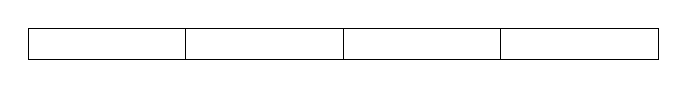
\begin{tikzpicture}[scale=\scalePic] {
    \allblue{(0,0),(2,0),(3,0)}
    \allred{(1,0),(4,0)}
    \allblue{(5,0),(8,0)}
    \allred{(6,0),(7,0),(9,0)}
    \allblue{(12,0),(13,0)}
    \allred{(10,0),(11,0),(14,0)}
    \allblue{(15,0),(17,0),(18,0)}
    \allred{(16,0),(19,0)}
    \grid{0}{5}{20}{0}{1}{1}
}\end{tikzpicture}
\end{center}

In each group of 5 points, there are $2^5 = 32$ possible colorings.\\
With $n=32$, and looking at each group as one ``point'', we have an infinite line of equally-spaced ``points'' colored with one of 32 colors.

From our earlier result, looking at $32+1=33$ of these ``points'' means that at least 2 of them will have the same color, which means that each element the group of 5 has the same color:

\begin{center}
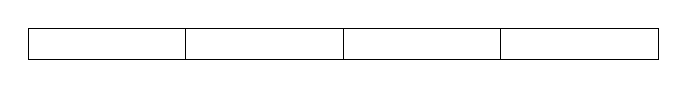
\begin{tikzpicture}[scale=\scalePic] {
    \allblue{(0,0),(2,0),(3,0)}
    \allred{(1,0),(4,0)}
    \allblue{(15,0),(17,0),(18,0)}
    \allred{(16,0),(19,0)}
    \grid{0}{5}{20}{0}{1}{1}
}\end{tikzpicture}
\end{center}

Looking at either of these 2 identical groups, we can find two points of the same color in the leftmost 3 points (call them $A$ and $B$ in each group), and the corresponding equally-spaced third point (also within the group of 5, call it $C$):

\begin{center}
\begin{tikzpicture}[scale=\scalePic] {
    \allblue{(0,0),(2,0),(3,0)}
    \allred{(1,0),(4,0)}
    \allblue{(15,0),(17,0),(18,0)}
    \allred{(16,0),(19,0)}
    \labelabove{0}{0}{A}
    \labelabove{2}{0}{B}
    \labelabove{4}{0}{C}
    \myboxes{(0,0),(2,0),(4,0)}
    \labelabove{15}{0}{A}
    \labelabove{17}{0}{B}
    \labelabove{19}{0}{C}
    \myboxes{(15,0),(17,0),(19,0)}
}\end{tikzpicture}
\end{center}

We also identify the equally-spaced group of 5 to the right of the 2 matching groups of 5. We care about the $C$ within this group:

\begin{center}
\begin{tikzpicture}[scale=\scalePic] {
    \allblue{(0,0),(2,0),(3,0)}
    \allred{(1,0),(4,0)}
    \allblue{(15,0),(17,0),(18,0)}
    \allred{(16,0),(19,0)}
    \labelabove{0}{0}{A}
    \labelabove{2}{0}{B}
    \labelabove{4}{0}{C}
    \myboxes{(0,0),(2,0),(4,0)}
    \labelabove{15}{0}{A}
    \labelabove{17}{0}{B}
    \labelabove{19}{0}{C}
    \myboxes{(15,0),(17,0),(19,0)}
    \labelabove{30}{0}{A}
    \labelabove{32}{0}{B}
    \labelabove{34}{0}{C}
    \myboxes{(34,0)}
}\end{tikzpicture}
\end{center}

Now we are fully set up.

Within the 2 left groups of 5, the 2 $A$'s have the same color, the 2 $B$'s have the same color, and the 2 $C$'s have the same color, since these groups are identical.\\
Additionally, $A$ and $B$ were chosen to have the same color.\\
Let $X$ be the color of these $A$'s and $B$'s, and $Y$ the color of these 2 $C$'s.\\

If $X=Y$, our line would satisfy the desired property.\\
In either one of these groups, $A$, $B$, and $C$ form 3 equally-spaced same-color points:
\begin{center}
\begin{tikzpicture}[scale=\scalePic] {
    \allblue{(0,0),(2,0),(3,0),(4,0)}
    \allred{(1,0)}
    \allblue{(15,0),(17,0),(18,0),(19,0)}
    \allred{(16,0)}
    \labelabove{0}{0}{A}
    \labelabove{2}{0}{B}
    \labelabove{4}{0}{C}
    \labelabove{15}{0}{A}
    \labelabove{17}{0}{B}
    \labelabove{19}{0}{C}
    \myboxes{(15,0),(17,0),(19,0)}
    \labelabove{30}{0}{A}
    \labelabove{32}{0}{B}
    \labelabove{34}{0}{C}
}\end{tikzpicture}
\end{center}

If $X\neq Y$, we form two different sets of equally-spaced points:

For our first set of points, we select the $A$ from the first group, $B$ from the second, and $C$ from the third.\\
As $A\rightarrow B\rightarrow C$ are equally spaced in a group, and the 3 groups are equally spaced, these 3 points are equally spaced.\\
Note that the first two points are both colored $X$.

\begin{center}
\begin{tikzpicture}[scale=\scalePic] {
    \allblue{(0,0),(2,0),(3,0)}
    \allred{(1,0),(4,0)}
    \allblue{(15,0),(17,0),(18,0)}
    \allred{(16,0),(19,0)}
    \labelabove{0}{0}{A}
    \labelabove{17}{0}{B}
    \labelabove{34}{0}{C}
    \myboxes{(0,0),(17,0),(34,0)}
}\end{tikzpicture}
\end{center}

For our second set of points, we select $C$ from all 3 groups.\\
As the groups are equally spaced, these 3 points are equally spaced.\\
Note that the first two points are both colored $Y$.

\begin{center}
\begin{tikzpicture}[scale=\scalePic] {
    \allblue{(0,0),(2,0),(3,0)}
    \allred{(1,0),(4,0)}
    \allblue{(15,0),(17,0),(18,0)}
    \allred{(16,0),(19,0)}
    \myboxes{(4,0),(19,0),(34,0)}
    \labelabove{4}{0}{C}
    \labelabove{19}{0}{C}
    \labelabove{34}{0}{C}
}\end{tikzpicture}
\end{center}

Now, considering the color of $C$ in the third group:

If it is $X$, the first set of points is equally-spaced with the same color:
\begin{center}
\begin{tikzpicture}[scale=\scalePic] {
    \allblue{(0,0),(2,0),(3,0)}
    \allred{(1,0),(4,0)}
    \allblue{(15,0),(17,0),(18,0)}
    \allred{(16,0),(19,0)}
    \allblue{(34,0)}
    \labelabove{0}{0}{A}
    \labelabove{17}{0}{B}
    \labelabove{34}{0}{C}
    \myboxes{(0,0),(17,0),(34,0)}
}\end{tikzpicture}
\end{center}

If it is $Y$, the second set of points is equally-spaced with the same color:
\begin{center}
\begin{tikzpicture}[scale=\scalePic] {
    \allblue{(0,0),(2,0),(3,0)}
    \allred{(1,0),(4,0)}
    \allblue{(15,0),(17,0),(18,0)}
    \allred{(16,0),(19,0)}
    \allred{(34,0)}
    \myboxes{(4,0),(19,0),(34,0)}
    \labelabove{4}{0}{C}
    \labelabove{19}{0}{C}
    \labelabove{34}{0}{C}
}\end{tikzpicture}
\end{center}

Thus, within $5*(2*(2^5+1)-1)$ points colored by 2 colors, we can find 3 equally-spaced ones with the same color.


\pagebreak
\subsection*{4 same-color corners of a square on an infinite 2-D lattice of 2 colors}

Yes, it is possible.
Proof:

\subsubsection*{3 corners of the square}

First, we show that, $\forall n\in\N$, given an infinite 2-D lattice of equally-spaced points, where each point is colored one of $n$ colors, it is always possible to find 3 points of the same color, where the 3 points form the top-left, bottom-left, and bottom-right corners of a square:

\begin{center}
\begin{tikzpicture}[scale=\scalePic] {
    \allblue{(0,0),(1,0),(0,1)}
}\end{tikzpicture}
\end{center}

In particular, $\exists f : \N \mapsto \N$ with $f(C) = G$ meaning that, within any $G \times G$ grid within the lattice colored by $C$ colors, the above pattern of 3 same-colored points can always be found.

Letting $C$ be constant, we prove the above statement by induction (but not on $C$).

$C=1$ holds trivially, as all points are the same color, so $f(1)=2$.

Observe the following process for $C=2$:

We first find how many adjacent points are needed in a line to guarantee 2 of the same color: $C+1$:

\begin{center}
\begin{tikzpicture}[scale=\scalePic] {
    \allblue{(0,0),(2,0)}
    \allred{(1,0)}
}\end{tikzpicture}
\end{center}

Now, for all possible pairs within this line, we append the point that would produce the desired patten of 3 points:

\begin{center}
\begin{tikzpicture}[scale=\scalePic] {
    \allblue{(0,0),(2,0),(1,1)}
    \allred{(1,0),(0,1),(0,2)}
}\end{tikzpicture}
\end{center}

For simplicity, we complete this into a square grid of side length $X=C+1$:

\begin{center}
\begin{tikzpicture}[scale=\scalePic] {
    \allblue{(0,0),(2,0),(1,1),(1,2),(2,2)}
    \allred{(1,0),(0,1),(0,2),(2,1)}
}\end{tikzpicture}
\end{center}

Now, partitioning our infinite grid into tiles of size $X \times X$, we treat each tile as having a unique color, with $T = C^{X^2} = C^{\left((C+1)^2\right)}$ possibilities. Even with this gigantic number of colors, we can still find two identical tiles, once we look at $T+1$ of them:

\begin{center}
\begin{tikzpicture}[scale=\scalePic] {
    \allblue{(0,0),(2,0), (1,1), (1,2), (2,2)}
    \allred{(1,0), (0,1), (0,2), (2,1)}
    \allblue{(9,0),(11,0), (10,1), (10,2), (11,2)}
    \allred{(10,0), (9,1), (9,2), (11,1)}
}\end{tikzpicture}
\end{center}

Now we start labeling points of interest. In both tiles, we find and label two points in the bottom row with the same color, and the third point within the grid that would complete the 3-point pattern.\\
If the third point has the same color as the bottom two, we have found the pattern. Thus we can assume that it has the other color (for this proof, we're only working with $C=2$ colors):

\begin{center}
\begin{tikzpicture}[scale=\scalePic] {
    \allblue{(0,0),(2,0), (1,1), (1,2), (2,2)}
    \allred{(1,0), (0,1), (0,2), (2,1)}
    \allblue{(9,0),(11,0), (10,1), (10,2), (11,2)}
    \allred{(10,0), (9,1), (9,2), (11,1)}
    \myboxes{(0,0),(0,2),(2,0),(9,0),(9,2),(11,0)}
}\end{tikzpicture}
\end{center}

We also find the point that, using the 2 ``third-points'' as the base of the pattern, would complete the pattern:
\begin{center}
\begin{tikzpicture}[scale=\scalePic] {
    \allblue{(0,0),(2,0), (1,1), (1,2), (2,2)}
    \allred{(1,0), (0,1), (0,2), (2,1)}
    \allblue{(9,0),(11,0), (10,1), (10,2), (11,2)}
    \allred{(10,0), (9,1), (9,2), (11,1)}
    \myboxes{(0,2),(9,2),(0,11)}
}\end{tikzpicture}
\end{center}

If this is the first color, we'd find the pattern:
\begin{center}
\begin{tikzpicture}[scale=\scalePic] {
    \allblue{(0,0),(2,0), (1,1), (1,2), (2,2)}
    \allred{(1,0), (0,1), (0,2), (2,1)}
    \allblue{(9,0),(11,0), (10,1), (10,2), (11,2)}
    \allred{(10,0), (9,1), (9,2), (11,1)}
    \allblue{(0,11)}
    \myboxes{(0,0),(11,0),(0,11)}
}\end{tikzpicture}
\end{center}

\begin{samepage}
If this is the second color, we'd find the pattern:
\begin{center}
\begin{tikzpicture}[scale=\scalePic] {
    \allblue{(0,0),(2,0), (1,1), (1,2), (2,2)}
    \allred{(1,0), (0,1), (0,2), (2,1)}
    \allblue{(9,0),(11,0), (10,1), (10,2), (11,2)}
    \allred{(10,0), (9,1), (9,2), (11,1)}
    \allred{(0,11)}
    \myboxes{(0,2),(9,2),(0,11)}
}\end{tikzpicture}
\end{center}
\end{samepage}

Thus, within a grid with side length $3*(2^9+1)$ on a 2-D lattice of 2 colors, we can always find three same-colored points that form the top-left, bottom-left, and bottom-right corners of a square.

Now, how do we prove this for arbitrary $C$ colors?

We give the general argument without rigor - see the final proof in this paper for rigor.\\
Repeat the above steps of:
\begin{itemize}
\item form a larger tile
\item find 2 horizontally-aligned identical copies of that tile
\item find the convergence point
\end{itemize}

Each time we repeat these steps, we either (A) find the desired pattern, or (B) force another color to be used at the new convergence point. Repeating this $C$ times, we run out of new colors, and find the desired pattern.\\
In the picture below, each outlined square is colored identically to each other square of that size. The space in between these squares is not to scale.
\begin{center}
\begin{tikzpicture}[scale=\scalePic*0.75] {
  \cppRun{\exe}{\\\{\\(0,0\\),\\(1,0\\)\\\} -\\> \\(0,1\\) blue 2 red 5 brown 9 orange}
}\end{tikzpicture}
\end{center}


\pagebreak
\subsubsection*{4\textsuperscript{th} corner of the square}

We proceed by an argument similar to the 3-corner proof:
\begin{center}
\begin{tikzpicture}[scale=\scalePic*0.75] {
  \cppRun{\exe}{\\\{\\(0,0\\),\\(1,0\\),\\(0,1\\)\\\} -\\> \\(1,1\\) blue 2 red 6 brown}
}\end{tikzpicture}
\end{center}

With 2 colors, there is some $G_{2,1}$ where a $G_{2,1} \times G_{2,1}$ grid will contain the 3-corner pattern.\\
For tiles of size $G_{2,1} \times G_{2,1}$, there are $2^{G_{2,1}^2}$ possible colorings of the tile.

There is some $X=G_{2^{G_{2,1}^2},1}$ where a $X \times X$ grid, colored by $2^{G_{2,1}^2}$ colors, will contain the 3-corner pattern.\\
Dividing the original grid into tiles of size $G_{2,1} \times G_{2,1}$, and taking a $X \times X$ grid of these tiles, we will find 3 identical tiles in the 3-corner pattern.

But the tiles are big enough that they themselves contain the 3-corner pattern, so we end up with a nested 3-corner pattern.\\
If the smaller 3-corner pattern also contained the same color in the upper-right corner of the square, we'd have a same-color square. So we assume it's the opposite color:
\begin{center}
\begin{tikzpicture}[scale=\scalePic*0.75] {
  \cppRun{\exe}{\\\{\\(0,0\\),\\(1,0\\),\\(0,1\\)\\\} -\\> \\(1,1\\) blue 2 red 6 white}
}\end{tikzpicture}
\end{center}

Then, looking at the upper-right convergence point, no matter which of the 2 colors it is, it completes a square.\\

Inner pattern color:
\begin{center}
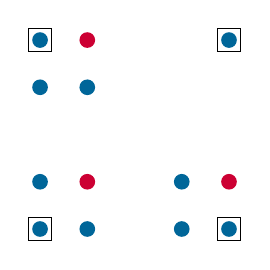
\begin{tikzpicture}[scale=\scalePic*0.75] {
\point{0}{0}{\blue}
\point{2}{0}{\blue}
\point{0}{2}{\blue}
\point{2}{2}{\red}
\point{6}{0}{\blue}
\point{8}{0}{\blue}
\point{6}{2}{\blue}
\point{8}{2}{\red}
\point{0}{6}{\blue}
\point{2}{6}{\blue}
\point{0}{8}{\blue}
\point{2}{8}{\red}
\point{8}{8}{\blue}
\mybigbox{0}{0}{1}{1}
\mybigbox{0}{8}{1}{1}
\mybigbox{8}{0}{1}{1}
\mybigbox{8}{8}{1}{1}
}\end{tikzpicture}
\end{center}

\pagebreak
Other color:
\begin{center}
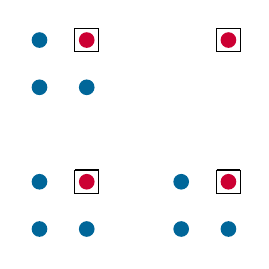
\begin{tikzpicture}[scale=\scalePic*0.75] {
\point{0}{0}{\blue}
\point{2}{0}{\blue}
\point{0}{2}{\blue}
\point{2}{2}{\red}
\point{6}{0}{\blue}
\point{8}{0}{\blue}
\point{6}{2}{\blue}
\point{8}{2}{\red}
\point{0}{6}{\blue}
\point{2}{6}{\blue}
\point{0}{8}{\blue}
\point{2}{8}{\red}
\point{8}{8}{\red}
\mybigbox{2}{2}{1}{1}
\mybigbox{2}{8}{1}{1}
\mybigbox{8}{2}{1}{1}
\mybigbox{8}{8}{1}{1}
}\end{tikzpicture}
\end{center}

Thus, given an infinite grid colored by 2 colors, we can always find 4 corners of a coordinate-aligned square of the same color within a $Y \times Y$ grid, where $Y = X * G_{2,1}$.

For illustrative purposes, see the following picture for finding 4 corners where the grid is colored by 4 colors (the black dot, as any of the 4 real colors, completes a square):
\begin{center}
\begin{tikzpicture}[scale=\scalePic*0.75] {
  \cppRun{\exe}{\\\{\\(0,0\\),\\(1,0\\),\\(0,1\\)\\\} -\\> \\(1,1\\) blue 2 red 6 brown 11 orange 24 black}
}\end{tikzpicture}
\end{center}


\pagebreak
\subsection*{General case}

Define a ``pattern'' as a finite sequence of $n$ distinct points:\\
$\left\{\mathbf{p_i} = \{x_{(i,1)}, ..., x_{(i,d)}\}\right\}_{i=1...n}$ with integer coordinates in any finite ($d$)-dimensional space.

We shall prove:

For any pattern in a $d$-dimensional space, where every point in the integer lattice is colored by one of a finite number of colors $C$ via some function $c(\mathbf{p})$, there exists a ``box size'' $B$ such that, in any $B \times B \times ... \times B$ box of points selected from the integer lattice, the pattern can be found (with some nonzero scaling factor $a$) with all points sharing the same color:\\
$\exists B \in \N, \forall \mathbf{q} \in \Z^{d}, \exists a \in \Z \setminus \{ 0 \}, \exists \mathbf{b} \in \Z^{d}$:
\begin{itemize}
\item $c(a \cdot \mathbf{p_1} + \mathbf{b}) = c(a \cdot \mathbf{p_2} + \mathbf{b}) = ... = c(a \cdot \mathbf{p_n} + \mathbf{b})$ (same color points)
\item $\forall 1 \leq i \leq n, \forall 1 \leq j \leq d, q_j \leq a \cdot x_{(i,j)} + b_j < q_j + B$ (pattern fits in the box)
\end{itemize}


\subsubsection*{Proof}
We induce on $n$, the number of points in the pattern.

$n=1$ is trivial: $B=1$ ($a=1$, $\mathbf{b} = \mathbf{q} - \mathbf{p_1}$).

For $n>1$, we use a new definition, and a new lemma:

We define a "Convergent $k$-repeating pattern" (for patterns $p$ with at least $2$ points) as a new pattern. It consists of the input pattern (except for its final point) repeated $k$ times, each with a different color. In all copies of the pattern, the final points converge at the same point.\\
For example, for this pattern $(0,0), (1,0), (2,1)$:
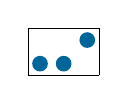
\begin{tikzpicture}[scale=\scalePic*0.75] {
  \point{0}{0}{\blue}
  \point{1}{0}{\blue}
  \point{2}{1}{\blue}
  \mybigbox{0}{0}{3}{2}
}\end{tikzpicture}

In the following picture, we have a convergent 3-repeating pattern of colors blue, red, and brown, that converges at the black point:\\
\begin{center}
\begin{tikzpicture}[scale=\scalePic*0.75] {
  \allblue{(-13,-13),(-26,-13)}
  \allred{(-12,-12),(-24,-12)}
  \allorange{(-9,-9),(-18,-9)}
  \allblack{(0,0)}
}\end{tikzpicture}
\end{center}

\pagebreak
Formally, given a pattern $p = \left\{\mathbf{p_i} = \{x_{(i,1)}, ..., x_{(i,d)}\}\right\}_{i=1...n}$, a convergent $k$-repeating pattern is:\\
$\exists \left\{ a_{i} \right\}_{i=1...k} a_{i} \in \Z \setminus \{ 0 \}, \exists \left\{ \mathbf{b_i} \right\}_{i=1...k} \mathbf{b_i} \in \Z^{d}$:
\begin{itemize}
\item $\forall 1 \leq i \leq k, \forall 1 \leq j < n$
\end{itemize}




\pagebreak
% \begin{tabular} with \cppRun as a cell element -> "fuck you" ~LaTeX
\begin{center}
$\vcenter{\hbox{

\begin{tikzpicture}[scale=\scalePic*0.75] {
  \point{0}{0}{\blue}
  \mybigbox{0}{0}{3}{3}
}\end{tikzpicture}
}}$
$\vcenter{\hbox{
\scalebox{2}{$\Rightarrow$}
}}$
$\vcenter{\hbox{

\begin{tikzpicture}[scale=\scalePic*0.75] {
  \point{0}{0}{\blue}
  \point{1}{1}{\blue}
  \mybigbox{0}{0}{3}{3}
}\end{tikzpicture}
}}$
$\vcenter{\hbox{
\scalebox{2}{:}
}}$
$\vcenter{\hbox{
\begin{tikzpicture}[scale=\scalePic*0.75] {
  \cppRun{\exe}{\\\{\\(0,0\\)\\\} -\\> \\(1,1\\) blue 1 red 1 brown 1 orange}
  \phantombox{2-32/2}{0}{32}{1}
}\end{tikzpicture}
}}$
\end{center}

\begin{center}
$\vcenter{\hbox{

\begin{tikzpicture}[scale=\scalePic*0.75] {
  \point{0}{0}{\blue}
  \point{1}{1}{\blue}
  \mybigbox{0}{0}{3}{3}
}\end{tikzpicture}
}}$
$\vcenter{\hbox{
\scalebox{2}{$\Rightarrow$}
}}$
$\vcenter{\hbox{

\begin{tikzpicture}[scale=\scalePic*0.75] {
  \point{0}{0}{\blue}
  \point{1}{1}{\blue}
  \point{1}{2}{\blue}
  \mybigbox{0}{0}{3}{3}
}\end{tikzpicture}
}}$
$\vcenter{\hbox{
\scalebox{2}{:}
}}$
$\vcenter{\hbox{
\begin{tikzpicture}[scale=\scalePic*0.75] {
  \cppRun{\exe}{\\\{\\(0,0\\),\\(1,1\\)\\\} -\\> \\(1,2\\) blue 1 red 3 brown 9 orange}
  \phantombox{27/2-32/2}{0}{32}{1}
}\end{tikzpicture}
}}$
\end{center}

\begin{center}
$\vcenter{\hbox{

\begin{tikzpicture}[scale=\scalePic*0.75] {
  \point{0}{0}{\blue}
  \point{1}{1}{\blue}
  \point{1}{2}{\blue}
  \mybigbox{0}{0}{3}{3}
}\end{tikzpicture}
}}$
$\vcenter{\hbox{
\scalebox{2}{$\Rightarrow$}
}}$
$\vcenter{\hbox{

\begin{tikzpicture}[scale=\scalePic*0.75] {
  \point{0}{0}{\blue}
  \point{1}{1}{\blue}
  \point{1}{2}{\blue}
  \point{2}{1}{\blue}
  \mybigbox{0}{0}{3}{3}
}\end{tikzpicture}
}}$
$\vcenter{\hbox{
\scalebox{2}{:}
}}$
$\vcenter{\hbox{
\begin{tikzpicture}[scale=\scalePic*0.75] {
  \cppRun{\exe}{\\\{\\(0,0\\),\\(1,1\\),\\(1,2\\)\\\} -\\> \\(2,1\\) blue 1 red 3.5 brown 11 orange}
  \phantombox{0}{0}{32}{1}
}\end{tikzpicture}
}}$
\end{center}

\pagebreak

\begin{center}
\begin{tikzpicture}[scale=\scalePic*0.75] {
  \cppRun{\exe}{\\\{\\(0,0\\),\\(0.5,1.5\\),\\(1,2.5\\),\\(2,2\\),\\(2.5,1\\),\\(1.5,0.5\\)\\\} -\\> \\(2.5,2.5\\) blue 3 red 10 brown}
}\end{tikzpicture}
\end{center}

\begin{center}
\begin{tikzpicture}[scale=\scalePic*0.75] {
  \cppRun{\exe}{\\\{\\(0,0\\),\\(0.5,1.5\\),\\(1,2.5\\),\\(2,2\\),\\(2.5,1\\),\\(1.5,0.5\\)\\\} -\\> \\(1.2,1.2\\) blue 3 red 10 brown}
}\end{tikzpicture}
\end{center}


QED $\blacksquare$

\end{document}